

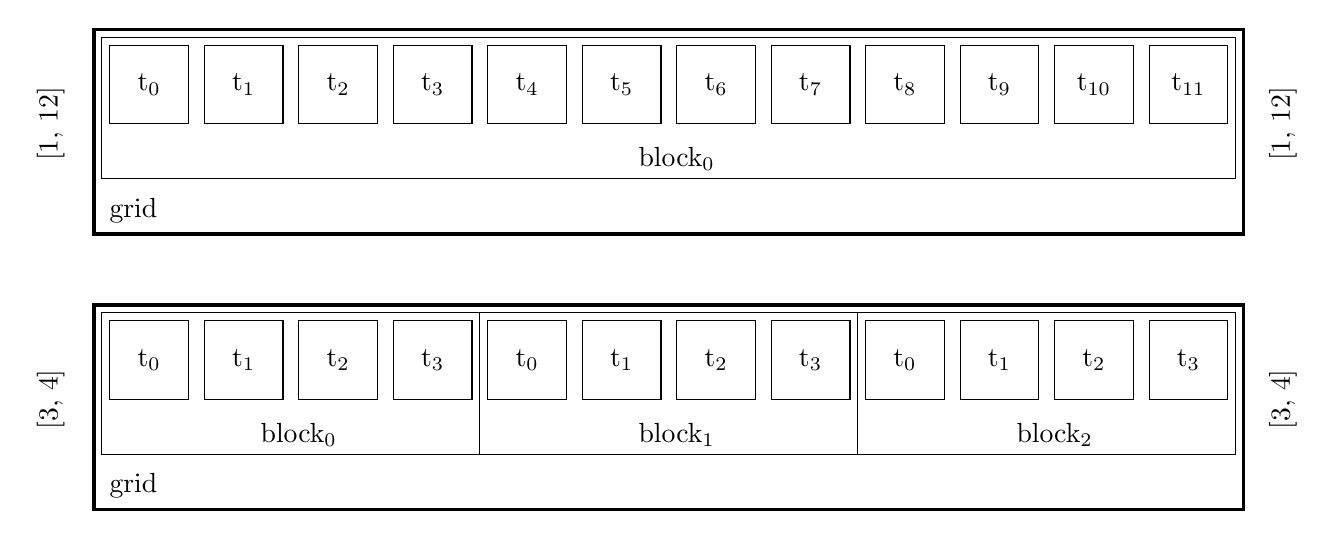
\begin{tikzpicture}[]


%%% DEFINITIONS %%%%%%%%%%%%%%%%%%%%%%%%%%%%%%%%%%%%%%%%%%%%%%%%%%%%%%%%%%%%%


% https://associatie.kuleuven.be/huisstijl/kleuren
\definecolor{blue1}{RGB}{82,189,236}
\definecolor{blue2}{RGB}{0,64,122}
\definecolor{blue3}{RGB}{31,171,231}
\definecolor{blue4}{RGB}{29,141,176}
\definecolor{blue5}{RGB}{17,110,138}
\definecolor{orange1}{RGB}{221,138,46}


\def\SignalY{2}
\def\GridOneY{-3.5}
\def\GridTwoY{0}
\def\MultiplierX{1.2}

\def\SquareSize{1}

\def\ThPoolCenterTwoX{2}
\def\ThPoolCenterTwoY{0}

\def\NumOfSamples{12}

\def\BlockDimX{4}


%%% DRAWING %%%%%%%%%%%%%%%%%%%%%%%%%%%%%%%%%%%%%%%%%%%%%%%%%%%%%%%%%%%%%%%%%



\foreach \b in {0,...,2} {
    \foreach \t in {0,...,3} {
        \pgfmathsetmacro{\res}{int(\t+\BlockDimX*\b)}
        \draw[black] ({(\t + \b * \BlockDimX) * \MultiplierX}, \GridOneY) rectangle ++ (\SquareSize, \SquareSize);
        \node at ({(\t + \SquareSize * \b * \BlockDimX) * \MultiplierX + \SquareSize/2}, \GridOneY + \SquareSize/2) {t$_{\t}$};
    }
    \draw[black] (-0.1 + \b * \MultiplierX * \BlockDimX, \GridOneY - 0.1 - 0.6) rectangle ++ (\SquareSize * \MultiplierX * \BlockDimX, \SquareSize + 0.2 + 0.6);
    \node at ({(\b + 0.5) * \MultiplierX * \BlockDimX}, \GridOneY - 0.45) {block$_\b$};
}


\draw[black, very thick] (-0.2, \GridOneY - 0.2 - 0.6 - 0.6) rectangle ++ (\SquareSize * \MultiplierX * \NumOfSamples + 0.2, \SquareSize + 0.4 + 0.6 + 0.6);
\node at (0.3, \GridOneY-1.1) {grid};

\node[rotate=90] at (-0.75, \GridOneY) {[3, 4]};
\node[rotate=90] at (\SquareSize * \MultiplierX * \NumOfSamples + 0.5, \GridOneY) {[3, 4]};




\foreach \x in {0,...,11} {
    \draw[black] (\x * \MultiplierX, \GridTwoY) rectangle ++ (\SquareSize, \SquareSize);
    \node at (\x * \MultiplierX + \SquareSize/2, \GridTwoY + \SquareSize/2) {t$_{\x}$};
}

\draw[black] (-0.1, \GridTwoY - 0.7) rectangle ++ (\SquareSize * \MultiplierX * \NumOfSamples, \SquareSize + 0.8);
\node at ({1.5 * \MultiplierX * \BlockDimX}, \GridTwoY - 0.45) {block$_0$};

\draw[black, very thick] (-0.2, \GridTwoY - 1.4) rectangle ++ (\SquareSize * \MultiplierX * \NumOfSamples + 0.2, \SquareSize + 1.6);
\node at (0.3, \GridTwoY-1.1) {grid};

\node[rotate=90] at (-0.75, \GridTwoY) {[1, 12]};
\node[rotate=90] at (\SquareSize * \MultiplierX * \NumOfSamples + 0.5, \GridTwoY) {[1, 12]};



\end{tikzpicture}